%% TCC - Monografia
%% Ci\^{e}ncia da Computa\c{c}\~{a}o - LCMAT - CCT - UENF, 2018
%% 

% definições
% arquiteturas
% arquitetura -> camadas e monolítico
% Ruby 
% Framework Rails
% deploy
% pipeline
% protocolos
% protocolos http e http/2
% ssl e TSL
% webservice
\chapter{Arquitetura de software}\label{cap2}

A arquitetura de software de modo geral tem por objetivo apresentar a comunicação entre cada camada do sistema, bem como, suas limitações, características e interfaces como bem definido por \cite{Sizo2010}. O trabalho tem por objetivo descrever as arquiteturas baseadas em camadas e microsserviços.

% focará em duas arquiteturas bem conhecidas no momento em que essa monografia está sendo escrita, são elas a arquitetura monolítico e a de Microsserviços.
Neste capítulo serão apresentadas diversas tecnologias, conceitos e definições que compõe as duas arquiteturas. Quando tratarmos de ferramentas iremos deixar claro que o intuito não é a ferramenta utilizada, mas os conceitos utilizados por elas, entretanto, deixaremos sempre em aberto a melhor tecnologia a ser aplicada, porém vamos utilizar algumas tecnologias como Node.js (http://nodejs.org), Firebase (http://firebase.google.com) e outras para conseguirmos chegar a conclusões concretas.

\section{Arquitetura}

\subsection{Decisões de Arquitetura}

Os desenvolvedores normalmente iniciam os projetos sem um planejamento de arquitetural adequada. Quando não se pensa no projeto como um todo e se desenvolve esse novo sistema de maneira desorganizada, a aplicação poderá sofrer grandes problemas conforme for crescendo, devido a falta de padrão. Naturalmente como já descreve  \cite{Richards2015} os projetos são desenvolvidos utilizando a arquitetura em camadas ou também chamada de arquitetura monolítica. Com uma arquitetura monolítica desorganizada, teremos módulos ou classes desorganizados e muitas responsabilidades em lugares inapropriados. Os engenheiros de softwares precisam entender e sempre justificar a decisão do uso daquela arquitetura.

% Seguindo essa estrutura o que acaba se tendo é uma quantidade de módulos ou classes com código desorganizado que não possuem responsabilidade e relacionamentos definidos entre os mesmos.
% Os engenheiros precisam conhecer as arquiteturas e sempre justificar as decisões do uso, principalmente quando se trata de uma arquitetura específica, como a de microsserviços.

Engenheiros de software e programadores implementam, corrigem, melhoraram, então repetem o ciclo de desenvolvimento. Após todas essas etapas, que são feitas por diversas vezes, a equipe inicia a fase de pensar em reconhecer ou melhorar a arquitetura que atende aquele sistema. Não é um processo fácil, a busca pela identificação da arquitetura ideal leva-se tempo, mas se faz necessário partir de um ponto inicial, \cite{Richards2015} descreve bem sobre essas etapas.

\subsubsection{Arquitetura em camadas ou monolítica}

A arquitetura em camadas/monolítica organizada em camadas horizontais, cada camada tem funções específica dentro do aplicativo (por exemplo, lógica de negócio, apresentação, persistência e banco de dados). No há uma quantidade ou tipo de camadas na arquitetura monolítica, mas naturalmente utiliza-se quatro camadas, são elas: lógica de negócio, apresentação, persistência e banco de dados como dito por \cite{Richards2015} como podemos verificar na figura \ref{fig:layered-architecture} . Em algumas descrições desse tipo de arquitetura pode se encontrar também três camadas como apresentação, camada de negócio e banco de dados. Aplicações menores normalmente seguem as três camadas, porém quanto maior e mais complexo mais camadas são acrescentada.


\begin{figure}[htbp]
    \hypertarget{arquitetura-camadas3}{%
        \caption{Arquitetura em camadas}
        \begin{center}
          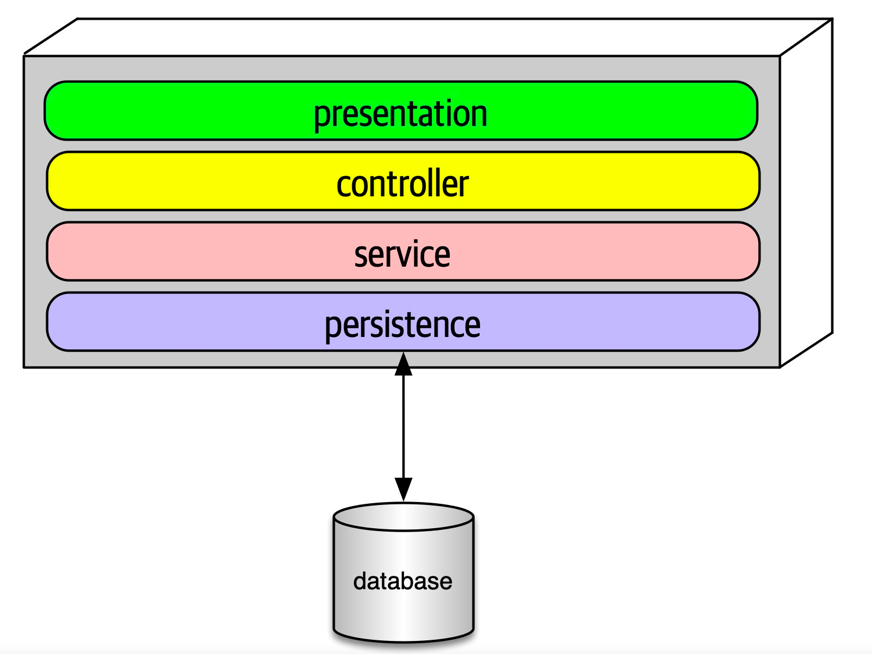
\includegraphics[width=10cm]{Monografia-FormatoLatex/Imagens/layered-architecture.png}
        \end{center}
    }
    \legend{Fonte: Imagem retirada do livro \citeonline[Cap.~4]{ford2020}}}.}}
    \label{fig:layered-architecture}
\end{figure}



As camadas na arquitetura tem função e responsabilidade específicas na aplicação. Podemos especificar algumas, como por exemplo a camada de apresentação que é responsável por lidar com toda a comunicação entre o sistema e o usuário que utiliza a aplicação, enquanto uma camada de negócios é responsável por executar regras de negócios específicas associadas à solicitação. Importante destacar que as camadas são abstrações e ela não precisa saber do sistema como um todo, ela só receber as informações que precisa para ser mostrada. Por exemplo, a camada de apresentação não precisa saber a regra de negócio, só exibir os dados para o usuário. \cite{Richards2015} explica muito bem as camadas, mas para um melhor entendimento, o cálculo é feito na camada de negócio, por exemplo 5 + 4, e a camada de apresentação só irá mostrar o valor final 9.

A arquitetura em camadas ou também conhecida como monolítica tem sido a mais utilizada por anos, haja visto que é uma das arquiteturas que mais temos conhecimento quanto a vantagens e desvantagens, pois há diversos artigos e também há uma experiência devido o tempo que trabalhamos com ela segundo \cite{Batista2018}.

A arquitetura monolítica pode ser descrita como um sistema centralizado, onde todas as responsabilidades e funcionalidades estão em um mesmo sistema, se por algum motivo um servidor pausar/falhar a aplicação inteira é afetada e nenhum usuário poderá utilizar a aplicação. Nesse tipo de arquitetura temos as algumas camadas que são elas: negócio, apresentação e dados, dependendo do modelo de arquitetura em camadas podemos ter outras como mostrado na figura \ref{fig:open-layer2}.

Podemos descrever algumas vantagens dessa tipo de arquitetura, por exemplo as camadas seguem uma hierarquia, as dependências são centralizadas, os códigos reutilizáveis e as regras de negócio também. Aplicações monolíticas são fáceis de serem desenvolvidas, afinal são ferramentas especializadas em uma única aplicação.

Como qualquer coisa específica, tem também suas desvantagens como descreve \cite{Batista2018}, a escalabilidade, agregação de novas tecnologias e a curva de aprendizado pode-se tornar alta e dependendo da regra de negócio, pode também ficar mais complexo, pois há uma grande base de código.

% \begin{figure}[htbp]
% \hypertarget{arquitetura}{%
% \caption{Arquitetura em camadas e o seu fluxo}

% \begin{center}
% 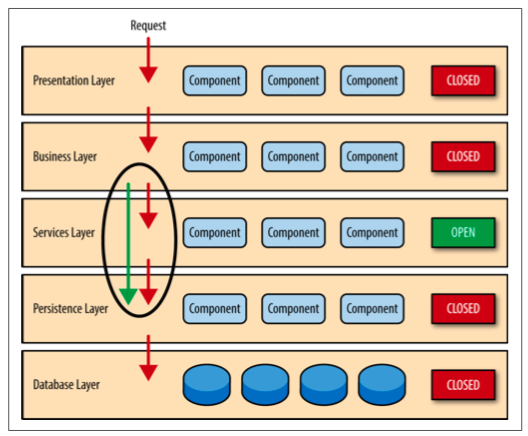
\includegraphics[width=10cm]{Monografia-FormatoLatex/Imagens/open-layer.png}
% \end{center}
% }
% \legend{Fonte: Imagem retirada do livro \citeonline[Cap.~1]{Richards2015}}.}}
% \label{mvc}
% \end{figure}


\begin{figure}[htbp]
    \hypertarget{arquitetura-camadas2}{%
        \caption{Arquitetura baseada em microsserviços}
        \begin{center}
          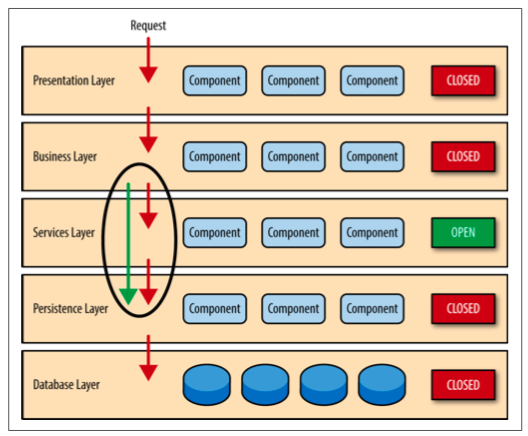
\includegraphics[width=10cm]{Monografia-FormatoLatex/Imagens/open-layer.png}
        \end{center}
    }
    \legend{Fonte: Imagem retirada do livro \citeonline[Cap.~1]{Richards2015}}.}}
    \label{fig:open-layer2}
\end{figure}



\subsubsection{Arquitetura de Microsserviços}


A arquitetura baseada em microsserviços ganhou muito destaca nos últimos anos por causa das grandes corporações que precisava escalar as suas aplicações de forma mais rápida e menos custosa e também para que suas equipem possam ter mais produtividade, haja visto que é melhor um colaborador trabalhar em um pequeno sistema, do que trabalhar com diversos sistemas complexos e que poderia gerar grandes prejuízos as empresas caso tenha alguma falha. \cite{Richards2015} explica que ainda há muitas dúvidas sobre o padrão baseado em microsserviços e a melhor forma de projetar esse tipo de arquitetura.

Buscaremos um modo para implementar esse tipo de arquitetura ao longo deste trabalho, porém é importante entender que há várias formas de se implementar a mesma arquitetura. Há conceitos que são pré requisitos para que a arquitetura seja considerada baseada em microsserviços, entretanto há formas mais elaboradas ou menos elaboradas. Cada micro serviço segue o princípio de responsabilidade única e tem como princípio que cada componente da arquitetura o isolamento desse sistema, com banco de dados próprio e comunicação via mensageria ou json por exemplo. Suas vantagens são perspetiveis em seus conceitos, onde podemos analisar brevemente que um sistema menor é mais simples de dar manutenção do que um sistema mais complexo, porém se faz necessário uma análise mais ampla as arquiteturas como \cite{Richards2015} expõe.

% Neste trabalho seguiremos um modo de implantação, porém é importante lembra-se que há várias formas de implementar, entretanto, há conceitos fundamentais para esse tipo de arquitetura. O conceito de software de responsabilidade única tem como princípio que cada componente da arquitetura de microsserviços é desenvolvida como uma unidade e há uma vantagem imediata, torna-se fácil o a entrega efetiva, construção de testes, escalabilidade e um alto grau de desacoplamento, pois a aplicação tem um contexto e esse contexto é uma aplicação pequena.

% A arquitetura baseada em microsserviços tem ganhado espaço em sistemas que necessitam escalar rapidamente como alternativa ou complemento a arquitetura em camadas ou também conhecida como monolítico. \cite{Richards2015} descreve que este tipo de arquitetura tem evoluindo, há ainda muitas dúvidas sobre esse padrão e no como implementar.
% Neste trabalho seguiremos um modo de implantação, porém é importante lembra-se que há várias formas de implementar, entretanto, há conceitos fundamentais para esse tipo de arquitetura. O conceito de software de responsabilidade única tem como princípio que cada componente da arquitetura de microsserviços é desenvolvida como uma unidade e há uma vantagem imediata, torna-se fácil o a entrega efetiva, construção de testes, escalabilidade e um alto grau de desacoplamento, pois a aplicação tem um contexto e esse contexto é uma aplicação pequena.

Com essa arquitetura necessitamos modificar a forma como desenvolvemos software de modo geral, como por exemplo pensar em componentes de serviços, no caso desse tipo de arquitetura a cada componente serviço pensado, teremos um sistema. A arquitetura pode conter um ou mais módulos ( por exemplo, classes em Ruby ou funções em Elixir) que representam um contexto de negócio único ( por exemplo, fornecer boletos para o usuário) ou mais ainda um aplicativo de negócios de grande porte (por exemplo, financeiro de uma empresa). \cite{Richards2015} explica que projetar o nível de granularidade dos componentes de serviço é um dos maiores desafios dos microsserviços.
% É importante pensar em componentes de serviços, que pode variar de um único módulo a uma grande parte do aplicativo. A arquitetura pode conter um ou mais módulos ( por exemplo, classes em Ruby ou funções em Elixir) que representam um contexto de negócio único ( por exemplo, fornecer boletos para o usuário) ou mais ainda um aplicativo de negócios de grande porte (por exemplo, financeiro de uma empresa). \cite{Richards2015} explica que projetar o nível de granularidade dos componentes de serviço é um dos maiores desafios de uma arquitetura de microsserviços.

Alguns conceitos chaves descritos por \cite{Richards2015} necessitam serem compreendidos, por exemplo os conceitos de sistema distribuídos. A arquitetura baseada em microsserviços segue os conceitos de sistemas distribuídos como já dito, isso significa que todos os componentes da arquitetura são desacoplados e acessados por meio de algum tipo de comunicação de acesso (por exemplo, AMQP, REST, SOAP, RMI, etc). É por isso que ela alcança as características de escalabilidade e implantação de forma superior a outras arquiteturas.

% É importante entender que essa arquitetura segue alguns conceitos chaves que \cite{Richards2015} cita, como ele é uma arquitetura com sistemas distribuídos, isso significa que todos os componentes da arquitetura são dissociados e acessados por meio de algum tipo de protocolo de acesso remoto (por exemplo, AMQP, REST, SOAP, RMI, etc). É por isso que ela alcança as características de escalabilidade e implantação de forma superior a outras arquiteturas.

Como já dito acima, não é pré-requisito a utilização de todos os componentens para se ter uma arquitetura baseada em microsserviços, porém para esse trabalho iremos utilizar um microserviço chamado API Gateway. O \cite{Florez2016} explica o quão benéfico é ter a API Gateway para lidar com diferentes solicitações de API, roteando-as para os microsserviços apropriados. Se você usa o API Gateway, projete e implemente-o com cuidado para evitar o acoplamento entre serviços. Cada microsserviço pode ter vários microcomponentes que podem ser separados em diferentes camadas. A \ref{fig:microsserviços} mostra esse tipo de microsserviço.

% \begin{figure}[htbp]
% \hypertarget{arquitetura}{%
% \caption{Arquitetura baseada em microsserviços}
% \label{microsserviços}
% \begin{center}
% 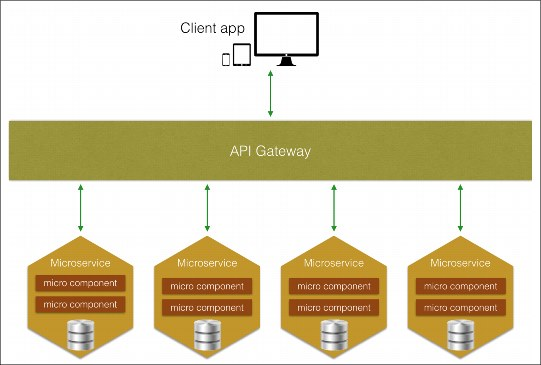
\includegraphics{Monografia-FormatoLatex/Imagens/api-gateway.jpg}
% \end{center}
% }
% \legend{Fonte: Imagem retirada do livro \citeonline[Cap.~2]{Florez2016}}.}}
% \end


\begin{figure}[htbp]
    \hypertarget{arquitetura-microservice1}{%
        \caption{Arquitetura baseada em microsserviços}
        \begin{center}
          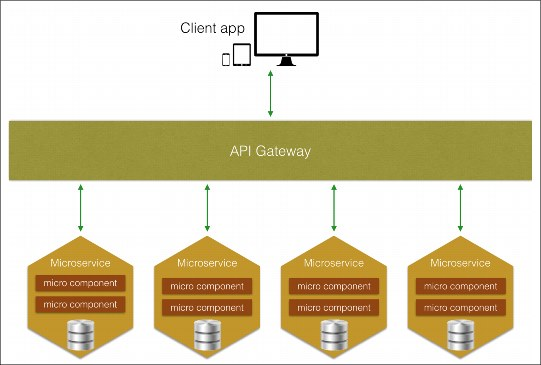
\includegraphics[width=10cm]{Monografia-FormatoLatex/Imagens/api-gateway.jpg}
        \end{center}
    }
    \legend{Fonte: Imagem retirada do livro \citeonline[Cap.~2]{Florez2016}}.}}
    \label{fig:microsserviços}
\end{figure}


 Sistemas baseados puramente na arquitetura de microsserviços seguem algumas características que \cite{TomasCerny2017} explora em seu artigo, são elas:
 
 \begin{itemize}
   \item O programa deve ter uma só tarefa e executar bem. Exemplo: gerador de PDF, ele só vai gerar PDF e fará muito bem essa função.
   \item A aplicação deve ser fácil de ser integrada a outros softwares. Qualquer aplicação que queira gerar PDF, poderá gerar facilmente.
   \item O gerador de PDF deve utilizar uma interface única com os outros sistemas, tudo de forma transparente para o usuário ou sistemas que irão utilizar.
 \end{itemize}

O \cite{Batista2018} define a arquitetura de Microsserviços como uma estrutura descentralizada, onde todas as camadas da aplicação ficam em servidores próprios e ambos se comunicam através das APIs. A forma de comunicação torna-os totalmente independentes e autônomos.

Uma descrição interessante é a dos autores do artigo \cite{Zhu2016} onde eles definem os microsserviços como sistemas que cada serviço é pequeno (daí o "micro") e que todos os desenvolvedores desses serviços entendam que estão trabalhando no mesmo sistema.

Esse tipo de arquitetura tem diversas vantagens como \cite{Batista2018} cita: 

\begin{itemize}
    \item Utiliza-se de comunicação leve e simples atráves do protocolo HTTP e com o HTTP version 2 a comunicação se tornou mais rápida.
    \item A utilização de qualquer linguagem de programação que o desenvolvedor queira utilizar.
    \item Permite experimentar e testar
    \item Bancos de dados diferentes
\end{itemize}

Com esse tipo de arquitetura há um ganho na diminuição de falhas, haja visto que são independentes, caso um sistema de pagamentos caia, o gerador de boletos, por exemplo continua funcionando. 
Entretanto esses benefícios não param por aí, como diz \cite{Tom2016} há diversos benefícios escondidos, ele dá alguns tópicos como: Inovação sem permissão, permissão para falhar, Interromper com confiança, você constrói, você mantém, acelera as descontinuações, testa de forma diferente, finaliza metadados centralizados, concentra a dor, caso tenha se interessado e deseja mais informações é sugerido que leia o artigo completo.

Uma das desvantagens que devemos nos preocupar quando estamos utilizando esse tipo de arquitetura é no contexto específico da aplicação e a complexidade entre a comunicação dos sistemas.


\subsection{ REST API}

REST significa REpresentational State Transfer, que é um estilo de arquitetura, e não um protocolo como definido muito bem no artigo \cite{Harber2019}.

\cite{Harber2019} descreve que a API é uma abreviação de interface de programa de aplicativo, que permite que os aplicativos se comuniquem. No caso da web, uma API é normalmente um conjunto de URLs que respondem com dados quando chamados da maneira correta e com as informações corretas.

Uma API REST é uma interface sem estado para seu aplicativo. No caso da pilha MEAN (Mongo, Express, Angular e NodeJS), a API REST é usada para criar uma interface sem estado para seu banco de dados, permitindo que outros aplicativos, como um SPA Angular, trabalhem com os dados. Em outras palavras, você cria uma coleção de URLs estruturadas que retornam dados específicos quando chamados, essa definição também é descrita por \cite{Harber2019}.


\subsection{Computação em nuvem}

A Computação em nuvem de forma simplista é levar ao usuário final, seja ele empresas ou pessoas físicas uma infraestrutura, plataforma ou software complexo, através de serviços simples e acessível de qualquer computador com um navegador instalado. Como \cite{Sousa2010} referencia no seu artigo, computação em nuvem é uma tendencia para os dias atuais e tem o objetivo entregar serviços sobre demanda, com pagamento baseado na utilização. Caso se interesse no assunto, o artigo do \cite{Sousa2010} é interessante para se aprofundar nesse conceito.

\cite{Hanjura2014} descreve que os serviços oferecidos pela computação em nuvem são divididos em diferentes modelos de serviço - infraestrutura como serviço (IaaS), plataforma como serviço (PaaS) e software como serviço (SaaS) como podemos verificar na figura \ref{fig:arquitetura-nuvem} . Essa classificação é feita para separar os diferentes tipos de serviços que um usuário pode adquirir para atender às necessidades de negócios em um ambiente de computação em nuvem.


% \begin{figure}[htbp]
% \hypertarget{arquitetura}{%
% \caption{ Alguns serviços suportados pela computação em nuvem }
% \label{fig:arquitetura-nuvem}
% \begin{center}
% 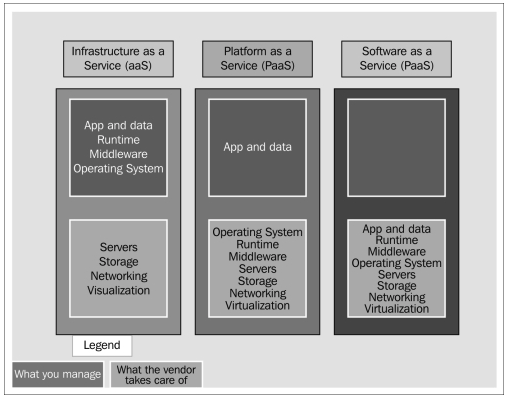
\includegraphics{Monografia-FormatoLatex/Imagens/computacao_em_nuvem.png}
% \end{center}
% }
% \legend{Fonte: Imagem retirada do livro \citeonline[Cap.~1]{Hanjura2014}}}.}}
% \end


\begin{figure}[htbp]
    \hypertarget{arquitetura-nuvem}{%
        \caption{Alguns serviços suportados pela computação em nuvem}
        \begin{center}
          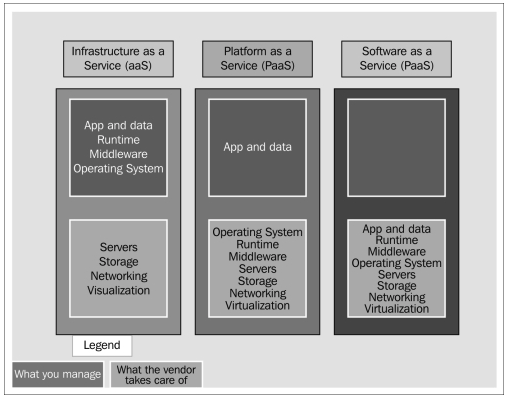
\includegraphics[width=10cm]{Monografia-FormatoLatex/Imagens/computacao_em_nuvem.png}
        \end{center}
    }
    \legend{Fonte: Imagem retirada do livro \citeonline[Cap.~1]{Hanjura2014}}.}}
    \label{fig:arquitetura-nuvem}
\end{figure}

A nuvem é classificada em alguns modelos de serviços. Cada modelo fornece um serviço distinto. Os modelos são IaSS, BaSS, PaSS e SaSS. Como \cite{Evangelista2016} cita em seu artigo a sigla em inglês significa Infrastructure as a Service (IaaS), Backend as a Service,  Plataform as a Service (PaaS) e Software as a Service (SaaS).

\subsection{Infrastructure as a Service (IaaS)}

É o tipo de modelo de serviço que permite ao usuário final utilizar capacidade de processamento, redes de dados, memória ram, SSD, sistema operacional e diversos componentes de hardware e rede. O IaSS permite gerenciar todos os recursos através de interfaces gráficas. Exemplo de IaSS: AWS, Google Cloud e Digital Ocean.

A definição de IaaS feita por \cite{Hanjura2014} é que o modelo de serviço em nuvem que permite ao usuário fornecer recursos de hardware virtualizado sob demanda. Fisicamente, esses recursos podem se espalhar por vários data centers, mantidos pelo provedor de serviços. Esses recursos incluem armazenamento virtual, conexões de rede e balanceadores de carga para o recurso de hardware provisionado. O usuário pode usar o recurso sob demanda e pagar por uso. Se o usuário precisar de mais recursos, o provedor poderá escalar automaticamente o hardware de acordo com a necessidade e vice-versa. Um bom exemplo de um provedor de IaaS é o Amazon Web Services (AWS - http: //aws.amazon.com). É o provedor de IaaS mais popular na nuvem. Rackspace (http://www.rackspace.com) é outro exemplo.


\subsection{Plataform as a Service (PaaS)}

É o modelo de serviço que levanta um servidor de diversas linguagens sem muito esforço. O usuário não tem acesso a infraestrutura, rede, dependências do sistema operacional e não precisa se preocupar com a atualização da mesma. Contrata só as configurações da plataforma.

A definição de PaaS feita por \cite{Hanjura2014} é que o modelo de serviço em nuvem que fornece as ferramentas para criar aplicativos de software na nuvem. Uma analogia próxima seria considerar o PaaS como um sistema operacional e um middleware do ambiente em nuvem. O PaaS fornece aos desenvolvedores a plataforma subjacente a ser usada para desenvolver seus aplicativos. Ele cuida do suporte a um idioma ou tecnologia específica que os desenvolvedores da pilha desejam usar. Muitos provedores de PaaS também permitem o dimensionamento sob demanda dos recursos subjacentes de computador e armazenamento, automaticamente, para liberar o usuário da nuvem da tarefa de alocar recursos manualmente. No PaaS, o consumidor do serviço controla a implantação e a configuração. O provedor PaaS provisiona os servidores, a rede e as necessidades computacionais do aplicativo de software. O modelo PaaS também permite uma arquitetura multitenant (definir isso) para que vários usuários possam usar o aplicativo da Web de maneira segura, escalável, simultânea e à prova de falhas. As sofisticadas soluções PaaS também fornecem um ambiente integrado de desenvolvimento de aplicativos da web, o que facilita a codificação colaborativa, o controle da fonte e a implantação. Heroku (http://www.heroku.com) e Google App Engine (http://cloud.google.com/AppEngine) são dois exemplos de plataformas PaaS de sucesso.

\cite{Hanjura2014} descreve que embora o PaaS seja inerentemente mais estável em comparação com o componente SaaS. PaaS evoluiu enormemente nos últimos anos e forneceu à comunidade de desenvolvedores ferramentas incríveis (menos adjetivo!) para trabalhar e implantar aplicativos distribuídos praticamente em pouco tempo.

\subsubsection{Heroku}

\cite{Hanjura2014} descreve o Heroku (http://www.heroku.com) como um dos principais fornecedores de PaaS no negócio de software em nuvem, provando ser a solução PaaS líder em pequenas e grandes empresas. Com melhorias consistentes e a filosofia de "conveniência" sobre "configuração", o Heroku se tornou a principal plataforma de desenvolvimento de aplicativos em nuvem para desenvolvedores. A filosofia da Heroku é permitir que os desenvolvedores se concentrem apenas em escrever aplicativos da Web e esquecer os servidores. O Heroku cuida magicamente da criação, implantação, execução e dimensionamento do aplicativo para o desenvolvedor sob demanda.


\cite{Hanjura2014} descreve o Heroku como uma plataforma de aplicativos em nuvem poliglota que oferece uma enorme flexibilidade na escolha de uma linguagem de programação apropriada para o desenvolvimento de aplicativos da web. O Heroku fornece suporte de plataforma para Ruby, Ruby on Rails, Java, Node.js, Clojure, Scala, Python e PHP a partir do início de 2013.

\subsection{Software as a Service (SaaS)}
É o modelo em que o usuário tem a aplicação disponível em tempo real através dos smartfones ou dos navegadores. O usuário não tem acesso a infraestrutura ou a plataforma, tudo é transparente para o usuário através de uma interface simples. O usuário só poderá configurar aspectos restritos da própria aplicação.

A definição de SaaS feita por \cite{Hanjura2014} é que o modelo SaaS da nuvem fornece software que você pode consumir do alcance do seu navegador da web. Não há necessidade de instalações complexas e demoradas. Abra um navegador, aponte para um URL e use o aplicativo apontado pelo URL. O que acontece nos bastidores está oculto ao usuário. O SaaS evoluiu consideravelmente na última década. Muitos provedores de SaaS tornaram obsoleto o software para desktop ou hospedado localmente. Tudo que você precisa é de um navegador e está pronto para usar qualquer aplicativo para fazer qualquer coisa. Sem dores de cabeça de atualizações de software, incompatibilidade de versão ou portabilidade de software. O serviço Gmail (http://gmail.com) do Google é uma das implementações de SaaS mais bem-sucedidas e conhecidas. O componente SaaS cresceu exponencialmente com empresas aproveitando a infraestrutura e a plataforma subjacentes para criar versões em nuvem da maioria de suas ofertas de produtos de software. Em 2013, quase todas as empresas que valem a pena ter uma versão SaaS de seus aplicativos populares de software disponíveis para clientes on-line.


\subsection{DevOps}

O DevOps é um conjunto de práticas ou uma cultura com o propósito de diminuir o tempo entre uma mudança feita e submetida em produção de forma a garantir a qualidade, seja em código ou seja em testes. O autor ainda descreve que toda mudança gera impactos nos processos, produtos, tecnologias utilizadas e estrutura organizacional, haja visto que estamos lidando com uma nova abordagem. A implantação dessa cultura não é fácil, muitas das vezes haverá tensões na organização e no negócio, pois terá que ser modificada a forma de trabalho diário como descreve \cite{Zhu2016}.

\cite{Zhu2016} descreve sobre os efeitos que o DevOps têm sobre os desenvolvedores ao longo do processo de desenvolvimento de software, ele lista alguns itens que valem a pena serem citados. São eles: 

\begin{itemize}
    \item Integração contínua é uma prática que deve ser utilizada e ela é o ato de submeter um código para um repositório central e o software executar os testes automatizados e subir para homologação ou produção sem que haja uma pessoa que cuide desse processo.
    \item Os sistemas são monitorados e após uma implementação, caso o haja alguma falha é possível reverter as alterações.
\end{itemize}

A utilização dessa cultura depende muito de diversas ferramentas, são elas: gerenciamento de contêineres, integração contínua, orquestração, monitoramento, implantação e teste. O \cite{Zhu2016} cita que cada vez mais, os engenheiros de software mantêm e configuram essas ferramentas.


\subsubsection{Docker}

Docker é uma aplicação que virtualiza os servidores, essa ferramenta foi desenvolvida para fornecer, via receita, um ambiente de forma rápida, seja para desenvolvimento ou produção. Todas às vezes ao inicializar um servidor necessitamos de um processo manual que se repete diversas vezes e que podemos automatizar e o docker torna esse processo simples. 

O Docker é considerada uma plataforma de virtualização em containers, ajuda os desenvolvedores a inicializar o ambiente sem esforço, basta ter a plataforma instalada localmente e conseguirá desfrutar dos benefícios de instalar sua aplicação, sem a necessidade de utilizar os arquivos da sua máquina física, em pouco minutos através do build da plataforma terá um ambiente totalmente configurado. O docker é uma tecnologia de código aberto, como \cite{Ouverney2017} descreve em seu artigo, durante o build é criado um container com todas dependências instaladas e a aplicação pronta para uso. Essa plataforma ajuda na implementação da arquitetura de microsserviços, pois cada aplicação fica isolada em um container, não afetando o funcionamento dos outros serviços.

\subsubsection{Testes automatizados}
 Durante o desenvolvimento de uma determinado sistema nos deparamos com diversos cenários de repetição de tarefas e, quando uma tarefa é repetitiva e pode ser automatizada, podemos automatizar esse processo, o que nos permite focar na resolução do problema que desejamos resolver. Os computadores fazem tarefas repetitivas melhor do que os humanos, o \cite{Bernardo2008} descreve em seu artigo, precisamos pensar em qualidade e nas inúmeras dificuldades quando se trata de questões humanas, então, porque não automatizar os testes, pois há processos repetidos que faríamos e poderemos falhar por falta de atenção em um dado momento.

A cultura DevOps já define em seus processos a automatização dos testes de software, \cite{Bernardo2008} define que os testes automatizados é uma técnica voltada a qualidade de software, onde uma alteração que possa quebrar o sistema, facilmente será percebida pelos desenvolvedores em poucos minutos. Existem alguns exemplos de testes, mas não se torna necessário descrever cada um deles, caso sinta-se curioso para saber mais sobre o artigo do \cite{Bernardo2008} lhe trará uma visão mais ampla sobre os tipos de teste.


\section{Tecnologias}

Nessa seção abordaremos algumas tecnologias e empresas que hospedam essas tecnologias para utilizarmos no dia a dia e de forma colaborativa.

\subsection{Git}

\cite{Beer2018} explica que o Git é um sistema de controle de versão. Esse tipo de software é projetado para acompanhar as alterações feitas nos arquivos ao longo do tempo. Ele explica ainda que o git é um sistema de controle de versão distribuído, o que significa que todos os que trabalham com um projeto no Git tem uma cópia do histórico completo do projeto, não apenas do estado atual dos arquivos.

\subsubsection{Github}

O Github é uma plataforma onde se pode fazer upload de uma cópia do seu repositório Git e de forma fácil toda sua equipe poderá fazer um clone do projeto e trabalhar simultaneamente no mesmo projeto como dito por \cite{Beer2018}. Ele ainda explica que o Github faz isso fornecendo um local centralizado para compartilhar o repositório, uma interface baseada na Web para visualizá-lo e recursos como fork, pull request, wiki do Github que permite especificar, discutir e revisar alterações com a sua equipe de forma mais eficaz. Caso queira saber mais informações basta acessar o site http://github.com.

\susubsection{Gitlab}

O Gitlab é uma plataforma de código aberto para armazenar uma cópia do seu repositório git, igualmente ao Github, podemos ter mais informações sobre o mesmo no \cite{Baarsen2014} ou no próprio site http://gitlab.com.

\subsection{Linguagem de Programação e Framework}

\subsubsection{ Node.js }

\cite{Herron2018} descreve o Node.js como uma nova e empolgante plataforma para desenvolvimento de aplicativos web e servidores de aplicativos. Essa tecnologia é detalhada como um projeto que trás extrema escalabilidade em aplicativos e em rede através de uma combinação engenhosa de JavaScript do lado servidor, I/O assíncrona e programação assíncrona. Ele é construído em torno de funções anônimas JavaScript e uma arquitetura orientada a eventos de encadeamento de execução única.

\cite{Herron2018} nos da uma informação importante sobre threads, o Node.js evita os threads por causa de sua complexidade. É dito que, com arquiteturas orientadas a eventos de thread única, o espaço ocupado na memória é baixo, o rendimento é alto, o perfil de latência de carga é melhor e o modelo de programação é mais simples. A plataforma Node.js está em uma fase de rápido crescimento, e muitos a veem como uma alternativa atraente às arquiteturas de aplicativos da web tradicionais usando Java, PHP, Python ou Ruby on Rails.

\subsubsection{React Native}

 React Native é uma estrutura de desenvolvimento de aplicativos na qual você usa tecnologias padrão da Web (ou, em alguns casos, algo semelhante às tecnologias padrão da Web) para criar seu aplicativo. Isso significa algo parecido com o HTML, JavaScript e CSS. O React Native é baseado na estrutura React do Facebook, uma estrutura popular de desenvolvimento da web. A diferença crítica entre os dois é que o React tem como alvo os navegadores da Web, enquanto o React Native tem como alvo os smartphones e seus sistemas operacionais como descrito por \cite{Zammetti2018}.

\subsection{Banco de dados}

\subsubsection{ MongoDB }

MongoDB é um banco de dados NoSQL para a Web moderna. NoSQL significa Not only SQL, é um termo cunhado por Carlo Strozzi em 1998, por seu banco de dados de código aberto que não seguia o padrão SQL, mas ainda era relacional, segundo \cite{Giamas2019}. Caso queira se aprofundar mais sobre o MongoDB, o mesmo conta com uma documentação completa no link https://docs.mongodb.com/manual/.

\subsubsection{ PostgreSQL }

\cite{Volkov2017} descreve o PostgreSQL como um sistema de gerenciamento de banco de dados relacional de objeto de código aberto. É executado nos sistemas operacionais mais modernos, incluindo Windows, MacOS e Linux. Está em conformidade com o SQL.

\subsection{Firebase}

O \cite{Yahiaoui2017} descreve o firebase como um BaaS, um back-end como serviço, com ele evitamos instalações e configurações que não iria agregar na solução do nosso problema para o momento.

O \cite{Yahiaoui2017} cita ainda que o Firebase é um BaaS com muitos recursos que facilita a criação dos projetos e elimina muitas tarefas tediosas e já fornecendo uma plataforma segura e bem construída que nos da simplicidade e escalabilidade de forma rápida.

\subsection{Firebase Realtime Database}


\cite{Yahiaoui2017} cita que o Firebase Realtime Database é o produto mais usado pelos desenvolvedores em toda a pilha de produtos disponíveis no Firebase. Ele oferece diversas funções como atualizações, inserções e exclusões de dados em tempo real.

\cite{Yahiaoui2017} detalha que a funcionalidade de transmissão integrada e uma API extremamente simples de usar torna o Realtime Database um recurso atraente. O interessante a se destaca que a APIs oferecem aos desenvolvedores a oportunidade de explorar as APIs em uma escala maior, independentemente do ecossistema e ambiente que eles estão usando. Além disso, o Firebase Realtime Database vem com suporte offline. Esse recurso entra em ação quando o aplicativo está em um estado de rede não tão confiável.


\subsection{Firebase Authentication}

Essa funcionalidade é uma das partes centrais de qualquer sistema e o \cite{Yahiaoui2017} descreve que a criação de um sistema de autenticação seguro acaba sendo um trabalho muito tedioso, mesmo que seja apenas e-mails e senhas.

Os aplicativos tendem a utilizar login com as redes sociais também e é um dos recurso mais utilizados e solicitados no cenário atual. É uma maneira rápida de fazer com que o usuário acesse o sistema como é descrito por \cite{Yahiaoui2017}.

\cite{Yahiaoui2017} descreve que o Firebase fornece métodos de autenticação múltipla, por exemplo email e senha, login social com as principais fornecedores Google, Facebook e etc.

\section{Trabalhos relacionados}

Nesta seção são mostrados alguns trabalhos relacionados sobre arquiteturas. Os trabalhos ajudaram na elaboração desse trabalho.

O autor \cite{Moreira2015} destaca as vantagens dos microsserviços e desvantagens dessa arquitetura, mostra na prática como criar uma arquitetura de microsserviço com Java Spring Boot. De modo geral o autor destaca que há diversas arquiteturas e a de microsserviços se encaixa em contextos específicos.

O artigo \cite{Chiaradia2018} aborda conceitos das áreas de gestão de relacionamento com o cliente, CRM Social e Web 2.0, enumerando as características e os benefícios. É proposta uma arquitetura de microsserviços para o sistema de CRM Social na qual o autor apresenta os fluxos de comunicação e se propõe a criação de um modelo para servir de base para futuras implementações. 

O objetivo do artigo \cite{TomasCerny2017} é conceituar as arquiteturas SOA (Service Oriented Architecture) quanto Microsserviços e mostrar as funcionalidades de cada arquitetura. O autor analisa a arquitetura quanto a performance, complexidade, tanto de implementação, quanto a uso nos dias atuais. 

Como \cite{Pahl2016} em seu artigo com o estudo de mapeamento dos métodos, técnicas e melhores práticas em arquitetura, com uma atenção particular à aplicação na nuvem. A revisão revela que a Microsserviços ainda está em um estágio formativo. É necessária uma avaliação mais experimental e empírica dos benefícios. Este estudo também demonstrou que a automatização e facilidade da arquitetura de Microsserviços em um cloud se torna necessário para extrair as vantagens que ela pode proporcionar.

O artigo \cite{Tom2016} descreve os diversos benefícios escondidos que a arquitetura de Microsserviço proporciona aos adeptos, no caso do artigo as empresas. Há algumas vantagens que não são claras no dia a dia, entretanto o artigo esclarece 8 pontos importantes que os administradores de modo geral poderão visualizar.

A arquitetura de Microsserviços  precisa ser monitorada, devido os micro sistemas estarem totalmente desacoplados, é necessário centralizar todas as informações e aí que o artigo \cite{Ghirotti2018} nos ajuda a entender a importância dessa arquitetura.

O artigo \cite{Raji2015} é importante, devido o mapeamento de visualização na área científica com a utilização da arquitetura de micro serviços, utilizando todos os conceitos da web 2.0. Um exemplo desse uso, em que o artigo retrata e o aumento da mobilidade, onde o mesmo pode ser utilizando em qualquer dispositivo e independente do sistema operacional, atingindo um público mais amplo e buscando ter um ecossistema mais rico, criando ferramentas e sites interativos. 

% \section{Análise das abordagens}

% Utilizando todos os artigos já listados até o momento e com a ideia de unir as duas arquiteturas analisamos que podemos unir ferramentas, arquitetura e o aprendizado.

% As ferramentas tem um papel importante, pois elas são o meio de torna a arquitetura viável. Nos diversos artigos lidos, algumas ferramentas são unanimes até o momento em que este trabalho está sendo escrito, mas o intuito não é prender a teoria das arquiteturas a ferramentas, mas sim a conceitos independentes delas, pois dado momento uma outra ferramenta, pode se tornar mais eficiente e mesmo assim os conceitos ainda continuaram sendo válidos.

% A arquitetura como tema central desse trabalho permite desenvolver software de qualidade em empresas. Os artigos se relacionam normalmente a contextos de negócios e não aos serviços públicos, o trabalho busca analisar os artigos e adaptar a realidade dos serviços públicos no Brasil.

% O trabalho deseja abordar também o aprendizado durante a criação de novas funcionalidades a projetos já existentes e o artigo \cite{Souza2009} explicita sobre o processo de aprender e as dificuldades que os alunos normalmente tem ao aprender uma linguagem de programação. Com a arquitetura que será conceituada, abordaremos também sobre a diminuição dessas dificuldades com a arquitetura que será proposta nos próximos capítulos.

% O autor \cite{Barker2017} nos disponibiliza diversas formas para metrificar a performance do nosso sistema, porém para esse trabalho o navegador será a nossa ferramenta principal. Os navegadores modernos nos disponibilizam um conjunto de ferramentas chamada de Dev Tools, como base faremos toda nossa analize com o dev tools do chrome.

% \section{Web Browser Developer Tools}

% Os navegadores web mais atuais incluem diversas ferramentas para os desenvolvedores web. Essas ferramentas são chamadas de Web Browser Developer Tools e navegadores como Chrome, Firefox, Safari, Edge ou Opera disponibilizam. Ferramentas que auxilia a identificar o fluxo das requisições e respostas, prioridades, dependências, o tempo e entender o Server Push. Nesse trabalho utilizaremos o \textbf{Chrome Developer Tools}.

% \subsection{Chrome Developer Tools}

% Nos últimos anos, o navegador Chrome ganhou adoção entre os desenvolvedores, em parte devido à crescente funcionalidades de suas ferramentas para desenvolvedores Web. Estar familiarizado com os recursos pode fornecer muitas vantagens para identificar diversos problemas técnicos como descreve \cite{Ludin2017}. Para acessar a ferramenta basta seguir os seguintes passos: Abra a ferramenta de desenvolvedor escolhendo Exibir -> Desenvolvedor -> Ferramentas de desenvolvimento no menu Chrome.

% Utilizaremos a aba Network para identificarmos todos os recursos que são carregados e o seu tempo para analisarmos o tempo de resposta das arquiteturas. A aba também nos proverá informações quando inserirmos um error que pare uma parte do sistema para identificarmos se o sistema continuará a responder a outra requisições. Como podemos visualizar na imagem \ref{fig:dev-tools} há uma aba chamada de Waterfall onde podemos analisar quais recursos foram carregados e em que ordem ocorreu.

% \begin{figure}[h]
%     \centering
%     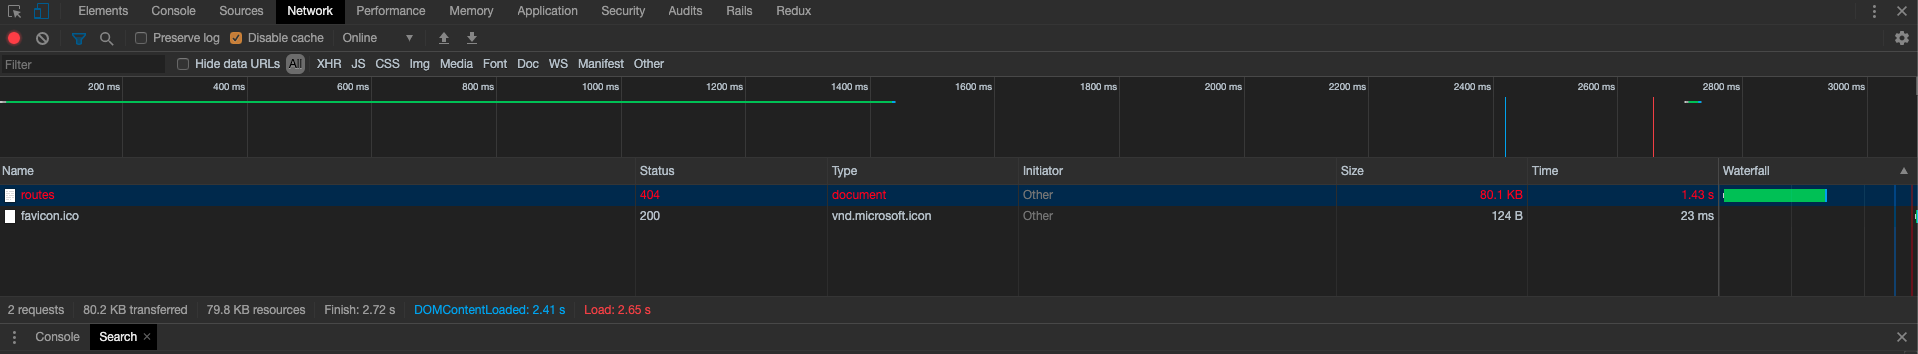
\includegraphics[width=12cm]{dev-tools.png}
%     \caption{ Imagens da aba Dev Tools do Chrome }
%     \label{fig:dev-tools}
% \end{figure}{}

% Há possibilidade de extrair diversos dados para a analisarmos como medida comparativa entre as arquiteturas, iremos utilizar a quantidade de requests feita por cada arquitetura, tamanhos dos dados transferidos, recursos recebidos e o tempo de finalização da página, esses dados serão extraídos no rodapé da ferramenta, como podemos observar na imagem \ref{fig:dev-tools2}

% \begin{figure}[h]
%     \centering
%     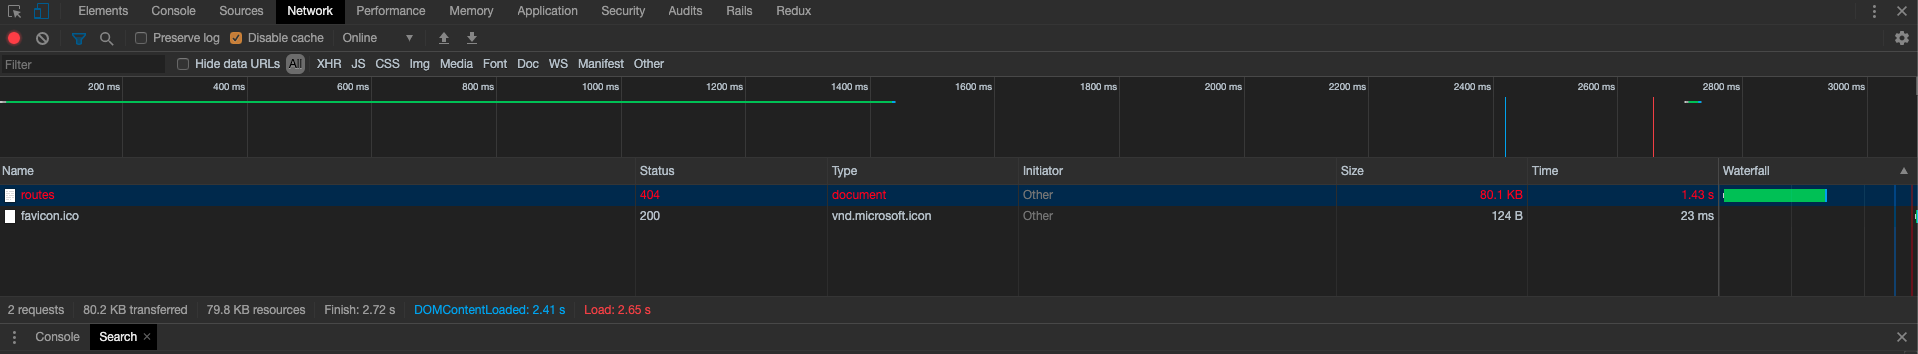
\includegraphics[width=12cm]{dev-tools.png}
%     \caption{ Imagens da aba Dev Tools do Chrome }
%     \label{fig:dev-tools2}
% \end{figure}{}